\label{chap:results}

%%....................................F.I.G.U.R.E.............................................
\begin{figure*}
	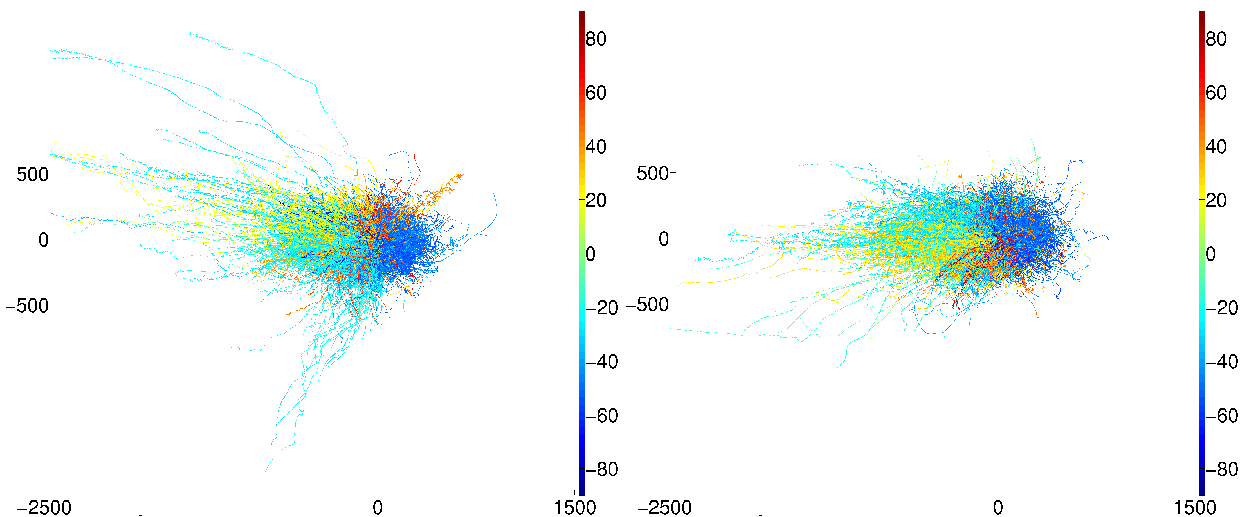
\includegraphics[]{defletcsBothCropd}
	\caption[\popSevenII tracks.]{Baseline-shifted tracks. Left: anticyclones. Right: cyclones. Color represents \textit{birth}-latitude. Thickness (hardly noticable) represents $\IQ$. Data is from a predecessor run to \popSevenII.}
	\label{fig:defletcsBothCropd}
\end{figure*}
%%....................................F.I.G.U.R.E.............................................


%\section*{resultsIntro}
%%....................................F.I.G.U.R.E.............................................
\begin{figure}
\includegraphics[width=\linewidth]{defl-age-aviI_shrunk2prepress}
\caption{\aviI: Baseline-shifted \textit{old} ($>\SI{500}{\day}$) tracks.}
\label{fig:defl-age-aviI_shrunk2prepress}
\end{figure}
%%...................................F.I.G.U.R.E.............................................
%%....................................F.I.G.U.R.E.............................................
\begin{figure}
\includegraphics[width=\linewidth]{defl-age-aviII_shrunk2prepress}
\caption{\aviII: (same as \cref{fig:defl-age-aviI_shrunk2prepress})}
\label{fig:defl-age-aviII_shrunk2prepress}
\end{figure}
%%....................................F.I.G.U.R.E.............................................

\newthought{Even}~though all of the computer program's bottle-necks are parllelized in \href{http://en.wikipedia.org/wiki/SPMD}{SPMD}, an application to more than a decade of high-resoultion \SSH~data still requires patience (say $\order{1}$ - $\order{2}$ days \footnote{depending on the number of cpu's and their frequencies.}). The most time-consuming of steps is the numerically arduous part of subjecting each of the vast number of found contours to the filtering procedure as described in \cref{S:04}.
The total number of final analyses was hence limited and it was therefor critical to carefully choose which method/parameters to use in order to maximize the deducible insights from the results.
For best comparability of the results with each other it was decided to agree on one complete set of parameters as a basis (\cref{tab:fixparams}), which would then be altered at key parameters.

\begin{itemize}
\setlength\itemsep{0mm}
\item 
The first run is an attempt to reproduce the results from \citet{Chelton2011}. The SSH-data for this run is therefor that of the \AVI~ product.
This method will be called \MI.
\item
The second run (\MII) is equivalent, except that this time the alternative $\IQ$-based shape filtering method as described in \cref{filter:shape} and the slightly different tracking-filter as described in \cref{item:checkDynamicIdentity} are used. \MII~is then fed with 7-day time-step \POP~data as well.
\item
To investigate what role spatial resolution plays, the \POP~data was remapped to that of the \AVI~data and fed to the \MI~method.
\item
Finally, to investigate the effects of resolution in time, an \MII-2-day-time-step run over \POP~data was executed. \TODO{popTwoII}
\item
Start and end dates were fix for all runs as the intersection of availability of both data sets.
\end{itemize}

%%

\begin{scriptsize}
\begin{margintable}
	\begin{tabularx}{\textwidth}{|X|X|}
	\hline
	time frame &  \displaydate{runsStart} till \displaydate{runsEnd}\\
	\hline
	scope & full globe ($80S:80N \;\; 180W:180E$) \\
	\hline
	\AVI geometry &   $641 x 1440$ true Mercator \\
	\hline
	POP   geometry &   $2400 x 3600$ \\
	\hline
	contour step   &   \contourstep \\
	\hline
	\end{tabularx}
	\begin{tabularx}{\textwidth}{|X|X|}
	\hline
	\textbf{thresholds} &  [all SI]  \\
	\hline
	max $\sigma/\Lr$ & \threshmaxRadiusOverRossbyL \\
	\hline
	min $\Lr$ & \threshminRossbyRadius \\
	\hline
	min $\IQ$ & \threshshapeiq \\
	\hline
	min number of data comprising found contour & \threshcornersmin \\
	\hline
	max(abs(Rossby phase speed)) & \threshphase \\
	\hline
		min amplitude & \threshamp \\
	\hline
	\end{tabularx}
	\caption{Fix parameters for all runs. \TODO{SI}}
\label{tab:fixparams}
\end{margintable}

%\newpage
%\begin{margintable}
	%\begin{tabularx}{1.1\textwidth}{|X||X|X|}
	%\hline
	 %& \MI & \MII   \\
	%\hline
%shape threshold & The distance between any pair of points within the connected region must be less than a specified maximum. & The Isoperimetric Quotient must be at least a specified minimum.\\
	%\hline
%Comparison of old to new eddy & ratio between new and old must lie between $0.25$ and $2.5$ for amplitude and area TODO ref & similar but with $\sqrt{\mathrm{area}/\pi}$ instead of area and the lower threshold as reciproke of the higher and vice versa.   TODO ref \\
	%\hline
	%\end{tabularx}
	%\caption{The two methods \MI and \MII.}
%\label{tab:MIMIIdiffs}
%\end{margintable}
\end{scriptsize}


\begin{infobox}[Method \MI]
The concepts used in this method are mostly based on the description of the algorithm described by \citet{Chelton2011} and all parameters are set accordingly. Basically \MI~is a modification of \MII~(which was completed first), with the aim to try to recreate the results from \citet{Chelton2011}.
It differs from \MII~in the following:
\begin{itemize}
\item \textbf{detection}\\
As mentioned in \cref{filter:shape}, the approach by \citet{Chelton2011} is to avoid overly elongated objects by demanding:
\begin{itemize}
\item high latitudes\\
The maximum distance between any vertices of the contour must not be larger than $400km$ for $\abs{\phi}>\deg{25}$.
\item low latitudes\\
The $400km$-threshold increases linearily towards the equator to $1200km$.
\end{itemize}
\item \textbf{tracking}\\
The other minor difference to \MII~is in the way the tracking algorithm flags eddy-pairs between time-steps as sufficiently similar to be considered successful tracking-candidates \\(see \cref{item:checkDynamicIdentity}).
In this method an eddy B from time-step $k+1$ is considered as a potential manifestations of an eddy A from time-step $k$ as long as both - the ratio of amplitudes (with regard to the mean of \SSH~within the found contour) and the ratio of areas (interpolated versions as discussed in TODO ref) fall within a lower and and an upper bound.
\end{itemize}
\label{box:MI}
\end{infobox}


\begin{infobox}[Method \MII]
The purpose of this variant is basically to test the conceptually different approach of using the \href{def:IQ}{isoperimetric quotient} to judge the shape of found contour-rings as sufficiently eddy-\textit{typical}. It also uses a slightly different tracking algorithm.
\begin{itemize}
\item \textbf{detection}\\
The $\IQ$-method. See \cref{fig:chiq5,fig:parAnalyIQ6,fig:parAnalyCH} and \cref{filter:shape}.
\item \textbf{tracking}\\
Conceptually similar to \MI, it is again vertical and horizontal scales that are compared between time-steps. Preferring a single threshold-value over one upper and one lower bound, a parameter $\xi$ was introduced that is the maximum of the two values resulting from the two ratios of amplitude respective $\sigma$, where either ratio is -if larger- its reciprocal in order to equally weight a decrease or an increase in respective parameter. In other words:
$\xi = \max{\left(\left[\exp{\abs{\log{R_{\alpha}}}}\; ; \;\; \exp{\abs{\log{R_{\sigma}}}} \right]\right)} $, where $R$ are the ratios.
%\TODO{this has been explained twice now...}
\end{itemize}
\label{box:MII}
\end{infobox}



\section{\mi~- 7 day time-step - \avi}
\label{section:aviI}
\newcommand{\run}[1]{#1-aviI}
\newcommand{\RUN}{\aviI:\;}
\newthought{The results } from the \MI -method are special in that they feature many long-lived eddies (see \cref{fig:histTrackCount-aviI,fig:tracks-age-aviI_shrunk2prepress,fig:defl-age-aviI_shrunk2prepress}),
some of which travelled more than $4000$ km west.
Tracks were recorded throughout the entire world ocean with the only exeptions being an approximately $\deg{20}$-wide stripe along the equator. The highest count of unique eddies is along the Antarctic Circumpolar Current \footnote{abbreviated ACC from here on.} with counts of more than $60$ individual eddy-visits per $\deg{1} \times \deg{1}$-cell. Further eddy-rich regions are the western North-Atlantic throughout the Gulf-Stream and North-Atlantic Current, \textit{Mozambique eddies} \citep{schouten2003eddies} at $\deg{20}$ South along the Mozambique coast, along the Agulhas Current and south of the Cup of Good Hope at $\sim \deg{40}$, along the coasts of Brazil, Chile and all along the Eastern, Southern and Western coasts of Australia (see \cref{fig:MapVisitsBoth-aviI}).

%%....................................F.I.G.U.R.E.............................................
\newthought{Eddies appear and disappear }  throughout the world ocean. For long-lived solid eddies there is a tendency to emerge along western coasts (see \cref{fig:birthsdeathsOneYearAndMore}).

\newthought{The scale } $\scale$ of tracked eddies is similar to that in \citet{Chelton2011}, yet generally smaller in high latitudes and slightly larger in low latitudes (see \cref{fig:Schelts-aviI}). It is larger than the first-mode baroclinic Rossby Radius by factor of at least $2$ and its meridional profile appears to be separable into two different regimes; one apparently linear profile in low latitudes and a steeper one equator-wards of $\sim \left| \deg{15} \right|$. Regionally, locations of high mesoscale activity appear to correlate with smaller eddy-scales (see \cref{fig:MapSigma-aviI}).

\newthought{The eastward zonal drift speeds } are slightly slower than the first-mode baroclinic Rossby-Wave phase-speed and agree well with the results from \citet{Chelton2011}. Propagation is generally west-wards except for regions of sufficiently strong eastward advection as in the ACC and North Atlantic Current (see \cref{fig:velZon-aviI,fig:Schelts-aviI}).

%%....................................F.I.G.U.R.E.............................................
\begin{marginfigure}
		\includegraphics[]{\run{histTrackCount}}
\caption[bla]{\RUN Final age distribtion. x-axis: [days], Left y-axis: [1000]}
\label{\run{fig:histTrackCount}}
\end{marginfigure}
%%....................................F.I.G.U.R.E.............................................
%%....................................F.I.G.U.R.E.............................................
\begin{figure}
	\includegraphics[]{\run{birthsdeathsOneYearAndMore}}
	\caption{\RUN Births are in blue and deaths in green. Size of dots scales to age squared. Only showing tracks older than one year.}
	\label{\run{fig:birthsdeathsOneYearAndMore}}
\end{figure}
%%....................................F.I.G.U.R.E.............................................
%%....................................F.I.G.U.R.E.............................................
%\begin{wrapfigure}{r}{0.6\textwidth}
\begin{marginfigure}
		\includegraphics[width=1\linewidth]{\run{MapVisitsBoth}}
		\caption{\RUN Total count of individual eddies per 1 degree square.}
		\label{\run{fig:MapVisitsBoth}}
\end{marginfigure}
%\end{wrapfigure}
%%....................................F.I.G.U.R.E.............................................
%%....................................F.I.G.U.R.E.............................................
\begin{figure}
		\includegraphics[]{\run{hist-sigmaAt-both}}
		\caption{\RUN \capS}
	\label{\run{fig:hist-sigmaAt-both}}
\end{figure}
%%....................................F.I.G.U.R.E.............................................

%%....................................F.I.G.U.R.E.............................................
\begin{figure*}
		\includegraphics[]{\run{MapSigma}}
		\caption{\RUN \capS}
	\label{\run{fig:MapSigma}}
\end{figure*}
%%....................................F.I.G.U.R.E.............................................

%%....................................F.I.G.U.R.E.............................................
\begin{figure*}
		\includegraphics[]{\run{velZon}}
		\caption{\RUN \capU }
	\label{\run{fig:velZon}}
\end{figure*}
%%....................................F.I.G.U.R.E.............................................

%\FloatBarrier

\section{\mii~- 7 day time-step - \avi}
\label{section:aviII}
\renewcommand{\run}[1]{#1-aviII}
\renewcommand{\RUN}{\AVI~-\MII:\;}


%%....................................F.I.G.U.R.E.............................................
\begin{figure}
\includegraphics[]{tracks-age-aviII_shrunk2prepress}
\caption{\MII: (see \cref{fig:tracks-age-aviI_shrunk2prepress})}
\label{fig:tracks-age-aviII_shrunk2prepress}
\end{figure}
%%....................................F.I.G.U.R.E.............................................


\newthought{The}~$\IQ$-based method results in approximately the same total amount of tracks as the \MI -method used in \cref{section:aviI} (see \cref{fig:histTrackCount-aviI,fig:histTrackCount-aviII}). The difference is that tracks here are generally much shorter, meaning that less eddies are detected at any given point in time.
The scale $\scale$ is now smaller than that from \citet{Chelton2011} for all latitudes in zonal- mean as well as median. Westward drift speeds are almost identical to those in \cref{section:aviI}.

%%....................................F.I.G.U.R.E.............................................
\begin{marginfigure}
		\includegraphics[]{\run{histTrackCount}}
\caption[bla]{\RUN Final age distribution. x-axis: [days], Left y-axis: [1000]}
\label{\run{fig:histTrackCount}}
\end{marginfigure}
%%....................................F.I.G.U.R.E.............................................
%%....................................F.I.G.U.R.E.............................................
\begin{figure}
	\includegraphics[]{\run{birthsdeathsOneYearAndMore}}
	\caption{\RUN Births are in blue and deaths in green. Size of dots scales to age squared. Only showing tracks older than one year.}
	\label{\run{fig:birthsdeathsOneYearAndMore}}
\end{figure}
%%....................................F.I.G.U.R.E.............................................
%%....................................F.I.G.U.R.E.............................................
%\begin{wrapfigure}{r}{0.6\textwidth}

%\end{wrapfigure}
%%%....................................F.I.G.U.R.E.............................................
%\begin{figure}
		%\includegraphics[]{\run{Schelts}}
		%\caption{\RUN Left: Zonal-mean drift speed (cyan) fit to Fig 22 of \protect{\citep{Chelton2011}} (Background) . Right: $\sigma$ and $L_{e}$ fit to Fig. 12 of their paper.}
	%\label{\run{fig:fSchelts}}
%\end{figure}
%%%....................................F.I.G.U.R.E.............................................

%\FloatBarrier

\section{\mii~- 7 day time-step - \pop}
\label{section:pop7II}
\renewcommand{\run}[1]{#1-pop7II}
\renewcommand{\RUN}{pop7-\MII: }

\newthought{The model data } delivers slightly more total tracks with a similar 2-fold dominance of cyclones over anti-cyclones (compare \cref{fig:histTrackCount-aviII,fig:histTrackCount-pop7II}). Similar to \aviII, very long tracks are fewer than via \aviI \footnote{\aviI~features $3000$ tracks that are older than $400$ days, while both \MII~methods have only $\sim1000$ of such.}. The regional pattern looks somewhat similar to the satellite patterns in terms of which regions feature the strongest eddy activity. With the exception of an unrealistic abundance of eddies right along the Antarctic coast  where no eddies were detected for the satellite data likely due to sea ice and/or the inherent lack of polar data due to the satellites' orbit-inclinations.

\newthought{The } more important difference between model- and satellite regional distributions is that the model results indicate significantly less eddy activity away from regions of strong \SSH~gradients, in the open ocean away from coasts and strong currents. The algorithm also detects hardly any eddy tracks in tropical regions (see \cref{fig:MapVisitsBoth}). This regional heterogenity in eddy-activity in the model data is also reflected in the distribtution of eddy amplitudes (see \cref{fig:TrackPeakampto_ellipseAntiCycsCrpd}).

\newthought{The scale $\scale$ } is generally smaller for the model-data-based analysis than for any satellite-based analyses, especially so in high latitudes.

\newthought{Westward drift speeds } look regionally similar to those from satellite data (\cref{fig:velZon-pop7II,fig:velZon-aviII}). In the zonal mean their magnitude is below those from satellite (see \cref{fig:ScheltsAll}).

%%....................................F.I.G.U.R.E.............................................
\begin{marginfigure}
		\includegraphics[]{\run{histTrackCount}}
\caption[bla]{\RUN Final age distribtion. x-axis: [days], Left y-axis: [1000]}
\label{\run{fig:histTrackCount}}
\end{marginfigure}
%%....................................F.I.G.U.R.E.............................................
%%....................................F.I.G.U.R.E.............................................
%~ %\begin{figure}
	%~ %\includegraphics[]{\run{birthsdeathsOneYearAndMore}}
	%~ %\caption{\RUN Births are in blue and deaths in green. Size of dots scales to age squared. Only showing tracks older than one year.}
	%~ %\label{\run{fig:birthsdeathsOneYearAndMore}}
%~ %\end{figure}
%%....................................F.I.G.U.R.E.............................................
%%....................................F.I.G.U.R.E.............................................
%\begin{wrapfigure}{r}{0.6\textwidth}
\begin{marginfigure}
		\includegraphics[width=1\linewidth]{\run{MapVisitsBoth}}
		\caption{\RUN Total count of individual eddies per 1 degree square.}
		\label{\run{fig:MapVisitsBoth}}
\end{marginfigure}
%\end{wrapfigure}
%%....................................F.I.G.U.R.E.............................................
\begin{figure*}
		\includegraphics[]{\run{MapSigma}}
		\caption{\RUN \capS}
	\label{\run{fig:MapSigma}}
\end{figure*}
%%....................................F.I.G.U.R.E.............................................

%%....................................F.I.G.U.R.E.............................................
\begin{figure*}
		\includegraphics[]{\run{velZon}}
		\caption{\RUN \capU}
	\label{\run{fig:velZon}}
\end{figure*}
%%....................................F.I.G.U.R.E.............................................

%%%....................................F.I.G.U.R.E.............................................
%\begin{figure}
		%\includegraphics[]{\run{hist-sigmaAt-both}}
		%\caption{\RUN TODO}
		%\label{\run{fig:hist-sigmaAt-both}}
%\end{figure}
%%%....................................F.I.G.U.R.E.............................................

%\FloatBarrier

%\section{\mii~- 7 day time-step - \pop~remapped to \avi~geometry}
%\label{section:p2aII}
%\renewcommand{\run}[1]{#1-p2aII}
\renewcommand{\RUN}{pop2aviso-\MII: }

\newthought{The model data }

\newthought{The scale $\scale$ }

\newthought{Westward drift speeds }
%%%....................................F.I.G.U.R.E.............................................
%\begin{marginfigure}
		%\includegraphics[]{\run{histTrackCount}}
%\caption[bla]{\RUN Final age distribtion. x-axis: [days], Left y-axis: [1000]}
%\label{\run{fig:histTrackCount}}
%\end{marginfigure}
%%....................................F.I.G.U.R.E.............................................
%\begin{wrapfigure}{r}{0.6\textwidth}
%\begin{marginfigure}
		%\includegraphics[width=1\linewidth]{\run{MapVisitsBoth}}
		%\caption{\RUN Total count of individual eddies per 1 degree square.}
		%\label{\run{fig:MapVisitsBoth}}
%\end{marginfigure}
%%\end{wrapfigure}
%%....................................F.I.G.U.R.E.............................................
\begin{figure*}
		\includegraphics[]{\run{MapSigma}}
		\caption{\RUN TODO}
	\label{\run{fig:MapSigma}}
\end{figure*}
%%....................................F.I.G.U.R.E.............................................
\begin{figure*}
		\includegraphics[]{\run{velZon}}
		\caption{\RUN TODO}
	\label{\run{fig:velZon}}
\end{figure*}

%\FloatBarrier

%%....................................F.I.G.U.R.E.............................................
\begin{marginfigure}
		\includegraphics[]{scat-UampAge-flat-pop7II}
		\caption{\RUN Small amplitude correlates with a short life and a broad translational speed spectrum. y-axis: translational speed $[cm/s]$, x-axis: amplitude $[cm]$, color: age [months].}
		\label{fig:scat-UampAge-flat-pop7II}
\end{marginfigure}
%%....................................F.I.G.U.R.E.............................................


\section{\mii~- 2 day time-step - \pop}
\label{section:popTwoII}
\TODO{run is finished. Results will be looked at / interpreted next week}

\subsection{\TODO{net U}}
\label{subsection:netU}	
\TODO{}

\FloatBarrier

%%%....................................F.I.G.U.R.E.............................................
\begin{figure}
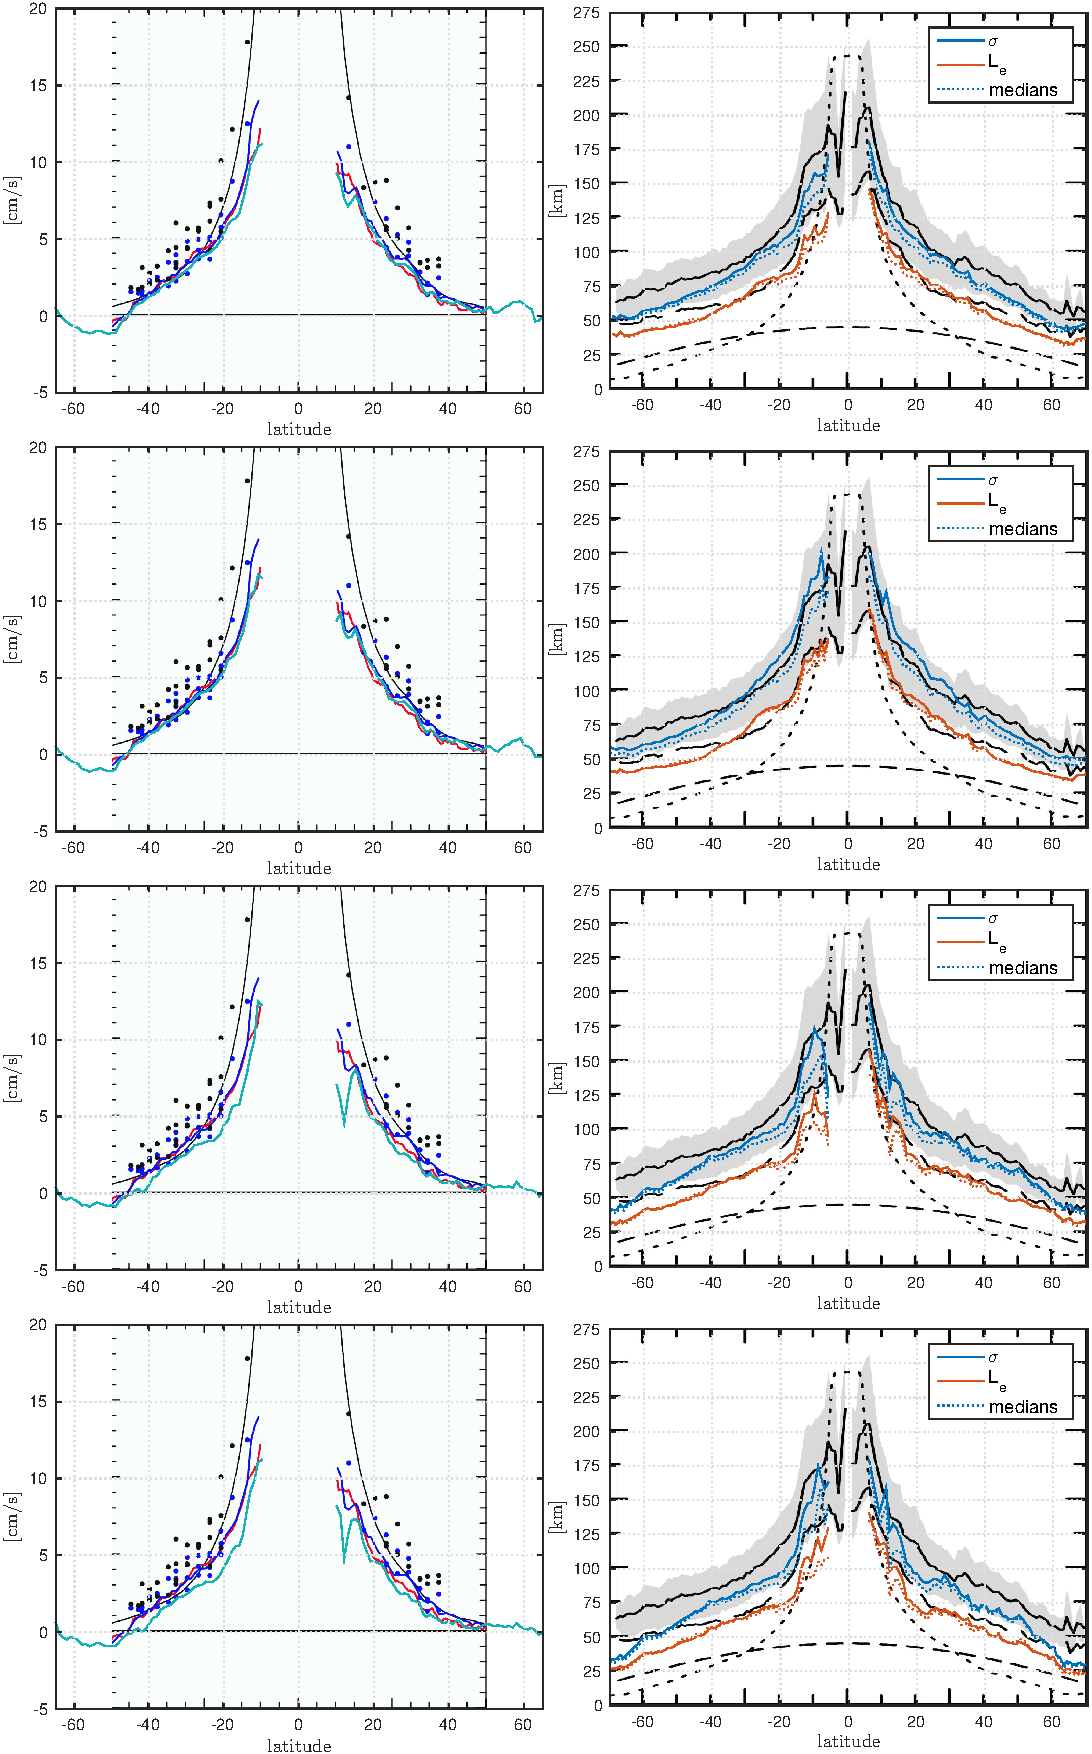
\includegraphics[]{ScheltsAll}
\caption{
Left: Zonal-mean drift speed (cyan) fit to Fig 22 of \protect{\citep{Chelton2011}} (Background).
Right: $\sigma$ and $L_{e}$ fit to Fig. 12 of their paper. Dotted lines are medians instead of means.
1st row: \protect{\aviII},
2nd row: \protect{\aviI},
3rd row: \protect{\pToaII},
4th row: \protect{\popSevenII}.
Note that for the very high latitudes ($>\abs{\deg{60}}$) the contrast between model and satellite data is further intensified by the lack of satellite data (see \cref{fig:MapSigma-aviII,fig:MapSigma-pop7II}) in those regions (sea-ice / orbit inclinations).
For a depiction without this effect see \cref{fig:sigmaSatDiffsINTRSCT}.
Regarding the underlying figures \citeauthor{Chelton2011} explain: [Left] \textit{The black dots are the Radon transforms of the $\ang{20} \times \ang{10}$ high-pass filtered SSH fields along [\ldots] zonal sections [\ldots] The red dots are the average along the propagation speeds of eddies with lifetimes $>16$ weeks within $\pm\ang{1.5}$ of latitude of the center latitudes of the same 45 zonal sections. The latitudinal profile of the global zonal average of the propagation speeds of all of the eddies with lifetimes $>16$ weeks is shown by the red line [\ldots]. The black line is the latitudinal profile of the zonally averaged westward phase speeds of long baroclinic Rossby waves.}
[Right] \textit{[\ldots] Meridional profiles of the average (solid line) and the interquartile range of the distribution of $\mathrm{L}_s$ (gray shading) in $\ang{1}$ latitude bins. The long dashed line is the meridional profile of the average of the e-folding scale Le of a Gaussian approximation of each eddy [\ldots]. The short dashed line represents the $\ang{.4}$ feature resolution limitation of the SSH fields of the AVISO Reference Series for the zonal direction [\ldots] and the dotted line is the meridional profile of the average Rossby radius of deformation [\ldots].}
}
\label{fig:ScheltsAll}
\end{figure}
%%....................................F.I.G.U.R.E.............................................


\FloatBarrier
